\section{Experiments on the synthetic tasks}
In this subsection we report some experiments which highlights the effects of the proposed techniques on the training process.

\subsection{The effect of the spectral initialization}

For this experiment we consider the temporal order task which has always been considered impossible to solve using the a plain version of the stochastic  gradient descent algorithm.
In \cite{advancesInOptimizingRnns}, for instance, are reported the rate of success of SGD and SGD modified with gradient clipping technique for such task with different input lengths. It shows that for sequences longer than 20 neither one of the algorithms can solve the problem. We repeated the same experiment, namely training the network varying the length\footnote{Here we refer as the length of the task to the minim length of the input sequences} of the input sequences, with the SGD algorithm modified with the gradient clipping technique using our initialization scheme. In figure \ref{fig:spectral_init_effect} are shown the number of iterations (means of 5 different runs with different random seeds) required to solve the problem for lengths in [50 100 150 200]. The important thing to notice is that, contrarily to what commonly believed, it is possible to train RNNs with SGD (with gradient clipping): not one of the runs for any length failed.

\begin{figure}
	\centering
	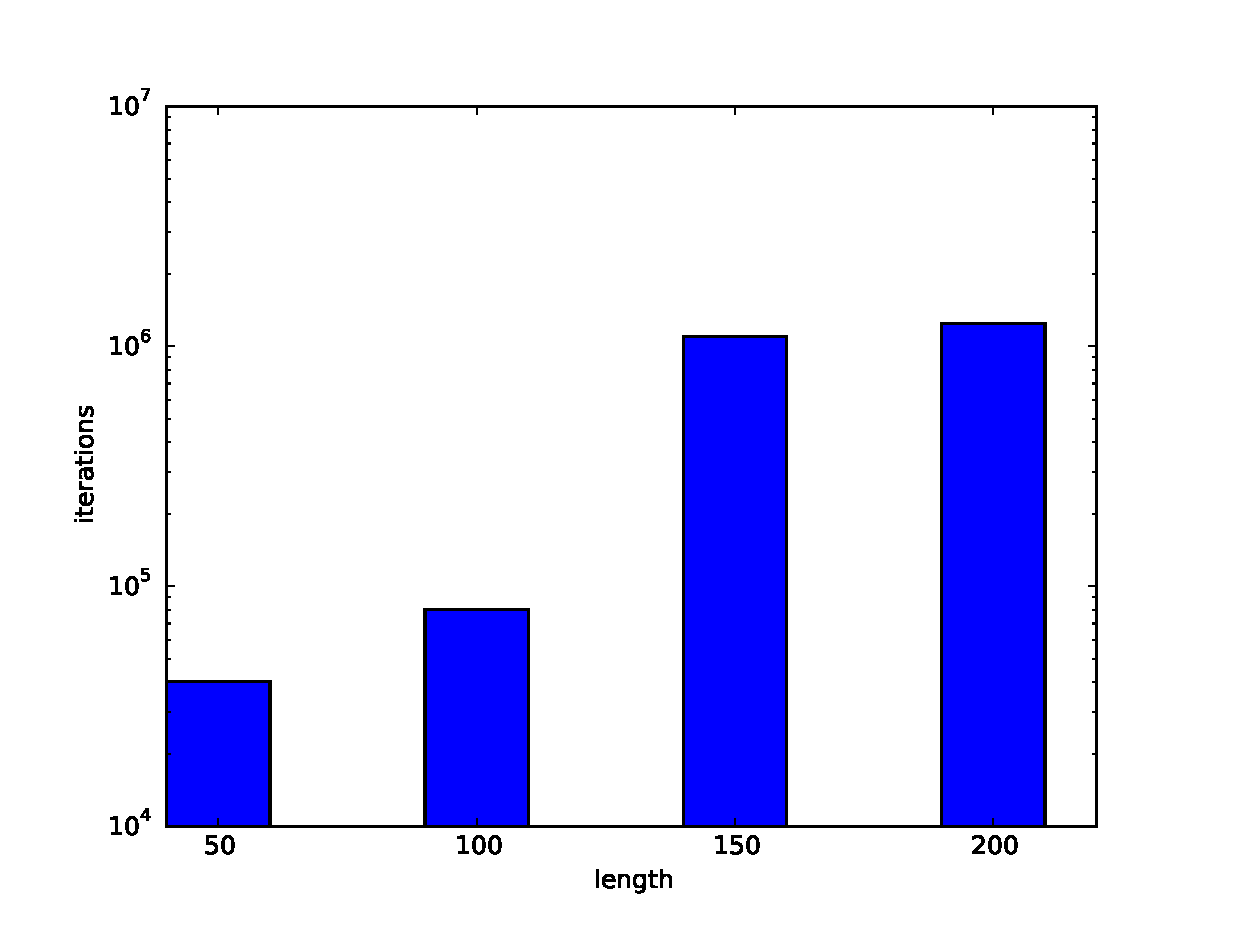
\includegraphics[width= 0.8\textwidth]{chapter4/spectral_init_exp.eps}
	\caption{Number of iterations (means of 5 different random seed) needed to solve the task for different lengths}
	\label{fig:spectral_init_effect}
\end{figure}
